\documentclass[11pt, oneside]{article}
\usepackage{geometry}
\geometry{letterpaper}
\usepackage{graphicx}
\usepackage{amssymb}
\usepackage{amsmath}
\usepackage{tikz}
\usepackage{tikz-qtree}
\usepackage{url}
\usepackage[T1]{fontenc}

\title{SICP Exercise 3.15}
\author{Yuchong Pan}

\begin{document}
\maketitle

The box-and-pointer diagram that shows the structure \url{z1} after evaluating \textbf{(set-to-wow! z1)} is given as follows.

\begin{figure}[h!]
    \centering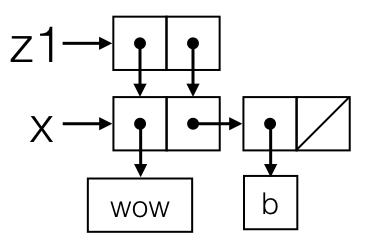
\includegraphics[width=7cm]{ex-3.15-1.png}
    \caption{Effect of \textbf{(set-to-wow! z1)}.}
\end{figure}

The box-and-pointer diagram that shows the structure \url{z2} after evaluating \textbf{(set-to-wow! z2)} is given as follows.

\begin{figure}[h!]
    \centering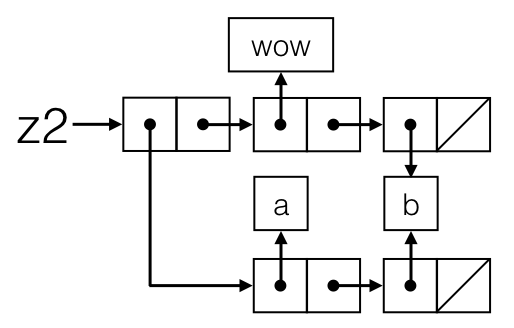
\includegraphics[width=7cm]{ex-3.15-2.png}
    \caption{Effect of \textbf{(set-to-wow! z2)}.}
\end{figure}

\end{document}
